% !TeX program = xelatex
\documentclass[11pt,a4paper]{article}
\usepackage[margin=25mm]{geometry}
\usepackage{amsmath,amssymb,amsthm}
\usepackage{booktabs}
\usepackage{tikz}
\usetikzlibrary{arrows.meta,positioning}
\usepackage[hidelinks]{hyperref}

\newtheorem{definition}{Definition}
\newtheorem{theorem}{Theorem}
\newtheorem{lemma}{Lemma}
\newtheorem{corollary}{Corollary}
\newtheorem{proposition}{Proposition}
\theoremstyle{remark}
\newtheorem{remark}{Remark}
\newcommand{\Sweep}{\mathcal S}
\newcommand{\remSweep}{\mathcal R}
\newcommand{\up}{\boldsymbol u}
\newcommand{\vp}{\boldsymbol v}

\title{Residual-Sweep Decomposition for Fixed-Path\\Coordination of Moving Objects}
\author{}
\date{November 20, 2026\\\small Initial working draft}

\begin{document}
\maketitle

\begin{abstract}
We study coordination of finitely many objects moving forward along fixed
paths. The formulation abstracts numerical time while retaining path order.
Swept occupied regions express potential interference independently of
particular speeds. We define residual sweeps and an undirected interference
graph, prove that its edges can only disappear under forward progress, and
show that its connected components can only split. Once separated, components
may execute independently without inter-component collisions, provided that
objects remain on their fixed paths and advance monotonically. Destination
occupancy is retained. These results establish a decomposition property; they
do not establish deadlock freedom or eventual completion within a component.
We also state the geometric conditions for merging consecutive tuple stages
and distinguish such merging from the controller's original departure rules.
\end{abstract}

\noindent\textbf{Keywords:} Sweep Volume; Collision Detection; Collision
Avoidance; Moving Objects; Multi Robot Path Planning.

\section{Scope and motivating question}

An overlap between two full-path sweeps identifies potential interference,
not a collision at a particular time. As objects advance, already passed
portions need no longer participate in future interference checks. Can the
resulting coordination problem separate into smaller independent problems?

Figure~\ref{fig:components} illustrates the property developed here. The
vertices represent objects, not road junctions. An edge means that two
\emph{residual sweeps} intersect. This is an interference graph, not a
directed precedence graph or a current wait-for graph.

\begin{figure}[htbp]
\centering
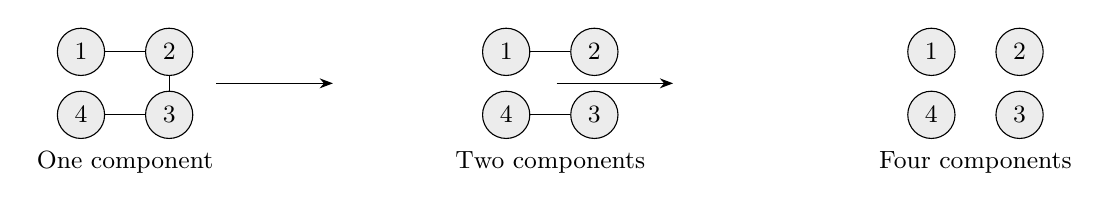
\begin{tikzpicture}[x=.8cm,y=.8cm,
 object/.style={circle,draw,fill=gray!15,minimum size=6mm,inner sep=1pt},
 every node/.style={font=\small},>=Stealth]
\foreach \id/\shift/\caption in {0/0/{One component},1/5.4/{Two components},2/10.8/{Four components}} {
  \begin{scope}[xshift=\shift cm]
  \foreach \i/\x/\y in {1/0/1,2/1.4/1,3/1.4/0,4/0/0}
    \node[object] (a\id-\i) at (\x,\y) {\i};
  \node at (.7,-.75) {\caption};
  \end{scope}
}
\draw (a0-1)--(a0-2)--(a0-3)--(a0-4);
\draw (a1-1)--(a1-2);
\draw (a1-3)--(a1-4);
\draw[->] (2.15,.5)--(4.0,.5);
\draw[->] (7.55,.5)--(9.4,.5);
\end{tikzpicture}
\caption{An illustrative sequence of component splits. Arrival of some objects
need not make every component a singleton: occupied destination footprints
can retain interference with other objects' residual paths.}
\label{fig:components}
\end{figure}

\paragraph{Assumptions.}
There are finitely many objects, each with a fixed ordered path and a fixed
occupancy model along that path. Objects may advance or wait, but path progress
never decreases. We do not add objects, assign new paths, or change footprint
dimensions or safety margins during the interval under consideration.
Geometric simplicity of a path is not required for the residual-set results:
even a later return to a spatial location remains part of its residual sweep.

\section{Related work and positioning}

\paragraph{Fixed-path coordination and asynchronous execution.}
O'Donnell and Lozano-P\'erez~\cite{odonnell1989} study two manipulators with
preplanned paths, variable execution durations, and explicit synchronization
commands. Their distinction between a geometric path and its execution in
time is directly relevant to our progress-based formulation. Leroy, Laumond,
and Sim\'eon~\cite{leroy1999} develop geometric coordination diagrams for
multiple mobile robots following independently computed paths. Our fixed-path
problem belongs to this established line of research rather than defining a
new general multi-robot planning problem.

\paragraph{Interference decomposition and independent groups.}
The interaction-graph construction in Leroy et al.~\cite{leroy1999} is a
particularly close precedent: vertices are robots, edges represent
intersecting traces, and connected components identify subgroups requiring
coordination. Connected-component decomposition is therefore not claimed as
new here. In cooperative pathfinding, Standley and Korf~\cite{standley2011}
exploit independence by planning groups separately and merging conflicting
groups when necessary. Their planning-time regrouping differs from the
execution-time splitting considered here under fixed paths, but independence
itself is an established computational principle.

\paragraph{Priorities, cycles, and robustness to delays.}
Gregoire, Bonnabel, and de La Fortelle~\cite{gregoire2015} use directed priority
graphs and coordination-space homotopy constraints for fixed-path robot
coordination. Their graph encodes ordering decisions; ours is an undirected
graph of potential residual interference. These graphs must not be conflated.
\v{C}\'ap, Gregoire, and Frazzoli~\cite{cap2016} prove safe, deadlock-free
execution under delaying disturbances. Their results are relevant to our
remaining completion-preservation question, but their guarantees do not
automatically transfer to a different departure rule.

\paragraph{Warehouse execution and merging movement commands.}
H\"onig et al.~\cite{hoenig2019} use an action dependency graph for robust
execution of warehouse MAPF schedules. Their model explicitly permits
combining consecutive forward actions into smooth motion while retaining
feedback for individual traversed edges (Section III-A). This closely relates
to our distinction between original control units and merged motion
commands. The present implementation should be compared with that execution
framework, not described as introducing this distinction for the first time.

\paragraph{Status of this draft.}
We provide a self-contained formulation of residual sweeps, conservative
reported progress, and the consequent refinement of interference components.
The set-containment and graph-refinement proofs below are elementary
consequences of the definitions; no priority-of-discovery claim is made for
them. Whether report-driven residual decomposition, its DEVS realization, or
a future completion-preserving controller provides a distinct research
contribution remains to be established by deeper comparison and evidence.

\section{Paths, occupancy, and subpath sweeps}

\begin{definition}[Ordered path and occupancy]
For each object $i\in\{1,\ldots,n\}$, let
\begin{equation}
 P_i:[0,1]\longrightarrow\mathcal Q_i,
 \qquad s_i=P_i(0),\quad e_i=P_i(1),
 \label{eq:path}
\end{equation}
be a continuous path in a configuration space. The parameter $u$ denotes
\emph{progress, not time}. Let $B_i(u)\subseteq\mathbb R^d$ be the nonempty
region occupied by the object at configuration $P_i(u)$.
For $0\le a\le b\le1$, its ordered subpath and subpath sweep are
\begin{equation}
 P_i^{[a,b]}=P_i|_{[a,b]},\qquad
 \Sweep_i[a,b]=\bigcup_{a\le u\le b}B_i(u).
 \label{eq:sweep}
\end{equation}
\end{definition}

A \emph{point sweep} is $\Sweep_i[a,a]=B_i(a)$. It represents occupancy while
waiting at that progress value; it is not an empty region. A full-path sweep
is $\Sweep_i[0,1]$. We treat contact as interference by using nonempty set
intersection as the test. Fixed geometric safety margins may be incorporated
in $B_i$.

For adjacent subpaths, write $\circ$ for ordered concatenation along the
original path, without introducing a spatial shortcut. Directly from
Definition~1,
\begin{equation}
 \Sweep_i[a,c]=\Sweep_i[a,b]\cup\Sweep_i[b,c]
 \quad(0\le a\le b\le c\le1).
 \label{eq:union}
\end{equation}

\paragraph{RMFS specialization.}
For an axis-aligned rectangular footprint translating along an axis-aligned
segment, the sweep is a rectangle. A piecewise axis-aligned path has a sweep
that is a union of such rectangles. When a robot rotates beneath a rack whose
orientation remains fixed, rack rotation adds no new rotational sweep.
The set results below do not require rectangular footprints or two dimensions.

\section{Paired paths, tuple paths, and sweep operations}

\begin{definition}[Tuple path]
A finite tuple path comprises ordered stages
\begin{equation}
 \mathcal T=(\mathcal P^{(1)},\ldots,\mathcal P^{(m)}),\qquad
 \mathcal P^{(k)}=(P_1^{[a_1^{(k)},b_1^{(k)}]},\ldots,
                   P_n^{[a_n^{(k)},b_n^{(k)}]}).
 \label{eq:tuple}
\end{equation}
Here each object's subpaths connect in their original order,
begin at progress $0$, and end at progress $1$:
\begin{equation}
 a_i^{(1)}=0,\quad b_i^{(k)}=a_i^{(k+1)},\quad b_i^{(m)}=1,
 \qquad a_i^{(k)}\le b_i^{(k)}.
 \label{eq:coverage}
\end{equation}
The case $n=2$ is a paired path. A point subpath, with $a_i^{(k)}=b_i^{(k)}$,
represents waiting during that stage.
\end{definition}

\paragraph{Point-sweep duplication.}
Copying and inserting a point subpath adds a waiting component to an
execution sequence. It does not alter the original geometric path or assign
a numerical waiting duration. Duplicating an arbitrary moving subpath is not
the waiting operation studied here.

\begin{proposition}[Safety of ordered tuple execution]
Suppose every distinct object pair has disjoint sweeps in each stage:
\begin{equation}
 \Sweep_i[a_i^{(k)},b_i^{(k)}]\cap
 \Sweep_j[a_j^{(k)},b_j^{(k)}]=\varnothing
 \qquad(i<j,\ k=1,\ldots,m).
 \label{eq:stage-safe}
\end{equation}
If stages execute sequentially and every stage can finish in finite time,
all objects complete their paths without collision in finite time.
\end{proposition}
\begin{proof}
During a stage, an object's occupied region lies within its stage sweep,
including when it waits at an endpoint. Equation~\eqref{eq:stage-safe}
therefore excludes collisions within that stage. The endpoint equalities
in~\eqref{eq:coverage} connect successive stages without changing path order.
A finite sum of finite stage durations is finite, and the final progress is
$1$ for every object.
\end{proof}

\paragraph{Merging consecutive stages.}
Two stages may be merged componentwise by concatenating each object's
adjacent subpaths. The merged sweep is their union, by~\eqref{eq:union}.
A conservative merge condition is
\begin{equation}
 \left(\Sweep_i[a_i^{(k)},b_i^{(k)}]\cup
       \Sweep_i[a_i^{(k+1)},b_i^{(k+1)}]\right)
 \cap
 \left(\Sweep_j[a_j^{(k)},b_j^{(k)}]\cup
       \Sweep_j[a_j^{(k+1)},b_j^{(k+1)}]\right)=\varnothing
 \quad(i<j).
 \label{eq:merge}
\end{equation}
If the stages are already individually safe, the additional tests are the
cross-stage terms, for all $i\ne j$:
\begin{equation}
 \Sweep_i[a_i^{(k)},b_i^{(k)}]\cap
 \Sweep_j[a_j^{(k+1)},b_j^{(k+1)}]=\varnothing.
 \label{eq:cross}
\end{equation}
Checking only selected or adjacent object pairs is insufficient. Under this
condition, merged ordered-stage execution satisfies the same safety argument
as Proposition~1, provided merged movements finish in finite time.

\begin{remark}[Commands and control units are distinct]
In the implementation, merging movement commands must not replace original
control boundaries or interference priorities with one long reservation.
The next original movement is judged first; only a currently permitted
consecutive prefix is combined into a command. A blocked later portion must
not delay an already permitted first movement. The safety of a merged stage
does not, by itself, prove correctness or completion of an asynchronous
controller that changes departure times.
\end{remark}

\section{Residual sweeps and interference groups}

\begin{definition}[Residual sweep and progress order]
At progress $u_i$, define the residual sweep of object $i$ by
\begin{equation}
 \remSweep_i(u_i)=\Sweep_i[u_i,1].
 \label{eq:residual}
\end{equation}
For progress vectors $\up,\vp\in[0,1]^n$, write $\up\preceq\vp$ if
$u_i\le v_i$ for every $i$. This is componentwise progress order, not an
assumption that all objects move synchronously.
\end{definition}

In particular,
\begin{equation}
 B_i(u_i)\subseteq\remSweep_i(u_i),\qquad
 \remSweep_i(1)=B_i(1)\ne\varnothing.
 \label{eq:occupancy}
\end{equation}
Completion removes the remaining movement, not the object's physical body.

\begin{lemma}[Residual containment]
If $u_i\le v_i$, then
\begin{equation}
 \remSweep_i(v_i)\subseteq\remSweep_i(u_i).
 \label{eq:containment}
\end{equation}
\end{lemma}
\begin{proof}
The progress interval $[v_i,1]$ is a subset of $[u_i,1]$. Taking the union of
the same occupied regions over a smaller index set cannot add any point.
\end{proof}

\begin{definition}[Residual interference graph and groups]
Define the undirected graph
\begin{equation}
 G(\up)=(V,E(\up)),\qquad V=\{1,\ldots,n\},\qquad
 \{i,j\}\in E(\up)\ \Longleftrightarrow\
 i\ne j\ \text{ and }\remSweep_i(u_i)\cap\remSweep_j(u_j)\ne\varnothing.
 \label{eq:graph}
\end{equation}
Its connected components are the residual interference groups. A singleton
component is an independent object. For display, non-singleton components
may be listed as groups and singletons listed separately.
\end{definition}

A pair without an edge can still belong to the same group through another
object. Group membership does not mean every pair in that group interferes.
Conversely, distinct components have no interfering cross-component pair.
This is the residual-path counterpart of the trace-interaction graph used
for decomposition in~\cite{leroy1999}.

\begin{theorem}[Edges can only disappear]
Under the fixed-path assumptions, if $\up\preceq\vp$, then
\begin{equation}
 E(\vp)\subseteq E(\up).
 \label{eq:edge-monotonicity}
\end{equation}
\end{theorem}
\begin{proof}
Take an edge $\{i,j\}\in E(\vp)$. There is a point in both
$\remSweep_i(v_i)$ and $\remSweep_j(v_j)$. By Lemma~1, that point also belongs
to both residual sweeps at $\up$. Thus $\{i,j\}\in E(\up)$.
\end{proof}

\begin{theorem}[Groups can only split]
If $\up\preceq\vp$, every connected component of $G(\vp)$ is contained in
exactly one connected component of $G(\up)$. Consequently, the component
containing any particular object cannot grow.
\end{theorem}
\begin{proof}
Every graph path in $G(\vp)$ also exists in $G(\up)$ by Theorem~1. Vertices
connected at $\vp$ must therefore belong to the same component at $\up$.
Uniqueness follows because connected components partition the unchanged
vertex set $V$.
\end{proof}

An edge deletion need not split a component: another graph path may still
connect its endpoints. Group size decreases only when enough edges disappear
to separate components.

\begin{corollary}[Finite structural change]
Starting from progress $\up$, there can be at most $|E(\up)|$ distinct edge
deletions. If there are initially $c$ components, there can be at most $n-c$
events that strictly increase the component count.
\end{corollary}
\begin{proof}
Each edge can disappear at most once, and none can appear. Each strict split
increases the component count by at least one, and that count is at most $n$.
\end{proof}

\section{What separation guarantees}

\begin{theorem}[Safe independent execution across groups]
Let $C$ and $D$ be distinct components of $G(\up)$. For every later progress
vector $\vp\succeq\up$ and all $i\in C$, $j\in D$,
\begin{equation}
 B_i(v_i)\cap B_j(v_j)=\varnothing.
 \label{eq:independent-safety}
\end{equation}
Thus independently chosen forward execution or waiting within the two groups
cannot produce a collision between those groups.
\end{theorem}
\begin{proof}
There is no edge between $i$ and $j$ at $\up$, so
$\remSweep_i(u_i)\cap\remSweep_j(u_j)=\varnothing$.
Each later occupancy is a subset of the corresponding earlier residual
sweep by~\eqref{eq:occupancy} and Lemma~1. Their intersection is therefore
empty, independently of their relative speeds or waiting durations.
\end{proof}

The quantification over arbitrary later progress vectors is what permits an
untimed statement about asynchronous execution. Physical time is needed to
evaluate durations and makespan, but not this inter-group exclusion result.

\begin{corollary}[Conditional composition of complete local executions]
If every component of $G(\up)$ has a collision-free execution of its residual
paths that completes in finite time, those executions can run independently
and together complete all residual paths without collision in finite time.
\end{corollary}
\begin{proof}
Internal collisions are excluded by each local execution's assumption;
cross-component collisions are excluded by Theorem~3. There are finitely many
components, so the maximum of their finite completion times is finite.
\end{proof}

The existence of those local complete executions is an assumption, not a
consequence of connected-component decomposition. A component can contain
deadlock, infeasible paths, or unsafe internal decisions.

\section{Reported progress and implementation correspondence}

A controller need not receive continuous position updates. Let $\hat u_i$
be the last conservatively established progress value. For reliable reports
on the fixed path, require
\begin{equation}
 \hat u_i\le u_i^{\mathrm{actual}},\qquad
 \hat u_i^{\mathrm{old}}\le\hat u_i^{\mathrm{new}}.
 \label{eq:reported-progress}
\end{equation}
Then the reported residual sweep contains both current occupancy and all
future occupancy along that path:
\begin{equation}
 B_i(v_i)\subseteq\remSweep_i(\hat u_i)
 \qquad(v_i\ge u_i^{\mathrm{actual}}).
 \label{eq:conservative-report}
\end{equation}
Delayed reports can retain unnecessary edges, but do not invalidate safe
separation. An erroneously advanced progress estimate can invalidate it.

\begin{table}[htbp]
\centering\small
\begin{tabular}{p{.27\linewidth}p{.65\linewidth}}
\toprule
Concept & Current RMFS correspondence \\
\midrule
Fixed ordered path & RoadMap's original Path and PathPosition data \\
Reported progress & RoadMap released\_progress, advanced by clearance and arrival reports \\
Residual sweep & Sweep of remaining\_subpath, including the current/destination footprint \\
Interference groups & Connected components recomputed from all residual sweep pairs \\
Control & TrafficManager retains original control units; group membership is currently tracking/display information \\
\bottomrule
\end{tabular}
\caption{Implementation correspondence; it does not substitute for a proof
of the complete departure algorithm.}
\label{tab:implementation}
\end{table}

These graph updates occur on reports, not on a periodic control-time loop.
Arrival at an intermediate command endpoint does not remove the remaining
original path. Arrival at the final endpoint leaves its point sweep.
The Viewer reads RoadMap state rather than inferring release independently.
The graph and report state are included in snapshot restoration.

\section{Boundaries and next proof obligations}

The present results establish residual-set containment, graph refinement,
and inter-group exclusion under fixed paths and monotone progress. They
do \emph{not} establish the following:
\begin{enumerate}
\item A feasible execution exists inside every remaining component.
\item A locally safe departure preserves eventual completion or prevents
      all later deadlocks.
\item A greedy sweep-merge policy finds every safe merge or minimizes makespan.
\item A finite collision-sampling experiment proves continuous-time safety.
\end{enumerate}
The next theoretical task is to state and prove conditions under which the
controller's asynchronous departure decisions preserve the feasibility of a
validated original tuple path. Runtime invariants and counterexamples should
be used to connect that proof to the actual implementation.
The comparisons with~\cite{cap2016,hoenig2019} should examine assumptions,
retained dependencies, feedback granularity, and liveness guarantees before
claiming a new execution method.

If paths, footprints, or participating objects change, recompute interference
and reconsider the decomposition. Previously separated groups may then merge;
Theorems~1--3 do not assert otherwise.

\begin{thebibliography}{9}

\bibitem{odonnell1989}
P.~A. O'Donnell and T. Lozano-P\'erez.
\newblock Deadlock-free and collision-free coordination of two robot manipulators.
\newblock In \emph{Proceedings of the IEEE International Conference on Robotics
and Automation}, pp.~484--489, 1989.
\newblock \url{https://lis.csail.mit.edu/pubs/tlp/coordination-o-donnell.pdf}.

\bibitem{leroy1999}
S. Leroy, J.-P. Laumond, and T. Sim\'eon.
\newblock Multiple path coordination for mobile robots: A geometric algorithm.
\newblock In \emph{Proceedings of the Sixteenth International Joint Conference
on Artificial Intelligence}, pp.~1118--1123, 1999.
\newblock \url{https://ijcai.org/proceedings/1999/0159.pdf}.

\bibitem{standley2011}
T.~S. Standley and R.~E. Korf.
\newblock Complete algorithms for cooperative pathfinding problems.
\newblock In \emph{Proceedings of the Twenty-Second International Joint
Conference on Artificial Intelligence}, pp.~668--672, 2011.
\newblock \url{https://doi.org/10.5591/978-1-57735-516-8/IJCAI11-118}.

\bibitem{gregoire2015}
J. Gregoire, S. Bonnabel, and A. de La Fortelle.
\newblock Robust multirobot coordination using priority encoded homotopic constraints.
\newblock arXiv:1306.0785v3, 2015. First submitted in 2013.
\newblock \url{https://arxiv.org/abs/1306.0785v3}.

\bibitem{cap2016}
M. \v{C}\'ap, J. Gregoire, and E. Frazzoli.
\newblock Provably safe and deadlock-free execution of multi-robot plans under
delaying disturbances.
\newblock arXiv:1603.08582, 2016.
\newblock \url{https://arxiv.org/abs/1603.08582}.

\bibitem{hoenig2019}
W. H\"onig, S. Kiesel, A. Tinka, J.~W. Durham, and N. Ayanian.
\newblock Persistent and robust execution of MAPF schedules in warehouses.
\newblock \emph{IEEE Robotics and Automation Letters}, 4(2):1125--1131, 2019.
\newblock \url{https://whoenig.github.io/publications/2019_RA-L_Hoenig.pdf}.

\end{thebibliography}

\end{document}
